\chapter{Indicadores de Qualidade do Solo e Funcionalidade Edáfica}
\label{cap:qualidade_solo}

\noindent\tagPratica
\vspace{4pt}

\begin{capObjetivos}
Ao concluir este capítulo, você será capaz de:
\begin{itemize}[leftmargin=1.5em, itemsep=2.5pt]
  \item Compreender o conceito de \textbf{Qualidade do Solo} sob a perspectiva da funcionalidade ecossistêmica integrada à dinâmica hidrológica e biológica (Doran; Parkin, 1994; Karlen et al., 1997; Vezzani; Mielniczuk, 2009).
  \item Selecionar um \textbf{Conjunto Mínimo de Dados} (\textit{Minimum Data Set}, MDS) equilibrado entre indicadores físicos, químicos e biológicos para diagnósticos ambientais.
  \item Calcular e interpretar densidade do solo ($D_s$), porosidade total ($P_t$), macro e microporosidade, matéria orgânica ($MO$), carbono orgânico total ($CO$) pelo fator de van Bemmelen, estoque de carbono, soma de bases ($SB$), $CTC$ e saturação por bases ($V\%$).
  \item Normalizar indicadores edáficos na escala de $0$ a $1$ segundo funções de desempenho (``quanto maior melhor'' e ``quanto menor melhor'') e computar passo a passo um \textbf{Índice de Qualidade do Solo (IQS)}.
  \item Interpretar gráficos radar multivariados comparando áreas de referência, áreas em recuperação com bioengenharia e áreas degradadas para fundamentar o Trabalho Prático Final.
\end{itemize}
\end{capObjetivos}

\begin{capRevisao}
Antes de avançar nos indicadores edáficos quantitativos, revise três bases anteriores da apostila:
\begin{itemize}[leftmargin=1.5em, itemsep=2.5pt]
  \item \textbf{Critérios de indicadores e modelo PEIR (Capítulo 10):} os atributos do solo funcionam como indicadores de \textbf{Estado (E)} sensíveis às pressões de uso da terra (compactação, desmatamento, manejo intensivo) e permitem monitorar a resposta de projetos de recuperação.
  \item \textbf{Morfopedologia e dinâmica água--solo--relevo (Capítulo 8):} a infiltração de água no perfil controla diretamente a partição entre recarga subsuperficial e escoamento superficial erosivo.
  \item \textbf{Fragilidade ambiental emergente (Capítulo 9):} solos rasos ou degradados fisicamente perdem capacidade de amortecer chuvas intensas, deslocando o sistema para a instabilidade ecodinâmica.
\end{itemize}
\end{capRevisao}

\etapa{3}{Fundamentação Teórica: Funcionalidade Edáfica, MDS e Cálculo do IQS}

\begin{boxSimbolo}[Vocabulário Técnico e Símbolos do Capítulo 11]
A \textbf{Qualidade do Solo (QS)} expressa a capacidade de um tipo específico de solo funcionar, dentro dos limites do ecossistema natural ou manejado, para sustentar a produtividade biológica, manter a qualidade da água e do ar e suportar a saúde dos habitats (Karlen et al., 1997). Para diagnosticar essa funcionalidade de forma operacional, seleciona-se um \textbf{Conjunto Mínimo de Dados (MDS, \textit{Minimum Data Set})}, composto por um grupo enxuto e não redundante de atributos físicos, químicos e biológicos com viabilidade analítica.

Na física do solo, $D_s$ representa a densidade do solo ($\text{g}\cdot\text{cm}^{-3}$) e $D_p$ indica a densidade de partículas (usualmente $2{,}65\text{ g}\cdot\text{cm}^{-3}$ para solos minerais quartzosos), enquanto $P_t$, $P_{\text{macro}}$ e $P_{\text{micro}}$ designam a porosidade total, a macroporosidade e a microporosidade ($\%$ em volume), acompanhadas pela taxa de infiltração básica ($TIB$, $\text{mm}\cdot\text{h}^{-1}$) e pela resistência à penetração ($RP$, $\text{MPa}$). Na química edáfica, $MO$ e $CO$ correspondem à matéria orgânica e ao carbono orgânico total ($\text{g}\cdot\text{kg}^{-1}$), relacionados pelo fator de van Bemmelen ($1{,}724$), ao passo que $SB$, $CTC$ e $V\%$ medem a soma de bases ($\text{cmol}_c\cdot\text{dm}^{-3}$), a capacidade de troca catiônica e a saturação por bases ($\%$). Na integração matemática, $S_i$ é a pontuação normalizada ($0$ a $1$), $w_i$ representa o peso atribuído ($\sum w_i = 1$) e $\text{IQS}$ corresponde ao Índice de Qualidade do Solo ($0$ a $1$).
\end{boxSimbolo}

\section{Conceito de Qualidade do Solo, Propriedades Inerentes e Tríade do MDS}

Historicamente, a ciência do solo privilegiou a avaliação da fertilidade química voltada à resposta imediata de lavouras a fertilizantes minerais. Na Análise Ambiental, essa abordagem isolada mostra-se insuficiente porque um solo rico em fósforo e potássio pode sofrer compactação severa sob tráfego de máquinas ou pisoteio, perdendo sua rede de poros maiores. Quando isso ocorre, a água da chuva encontra resistência na superfície, forma enxurrada erosiva, arrasta sedimentos para os rios e reduz a recarga do lençol freático.

A partir da década de 1990, Doran e Parkin (1994) e Karlen et al. (1997) consolidaram o conceito moderno de \textbf{Qualidade do Solo}, centrado em cinco funções ecossistêmicas interdependentes. O solo regula e particiona o fluxo de água (controlando infiltração, armazenamento e drenagem), sustenta a biodiversidade e a atividade biológica subterrânea, filtra e tampona poluentes orgânicos e inorgânicos, cicla nutrientes ao mesmo tempo em que estoca carbono orgânico, e oferece suporte físico estável às raízes e às obras humanas. No Brasil, Vezzani e Mielniczuk (2009) enfatizam que essa qualidade emerge da interação contínua entre estrutura física (agregação), dinâmica da matéria orgânica e organismos vivos, exigindo comparação direta com um \textbf{solo de referência} sob vegetação nativa da mesma classe pedológica e condição climática.

Para diagnosticar se um solo perdeu funcionalidade por ação humana ou se determinada característica é natural daquele ambiente, distingue-se o potencial herdado da condição dinâmica atual (Figura~\ref{fig:triade_mds_funcoes}). As \textbf{propriedades inerentes} (textura areia--silte--argila, mineralogia da fração argila, profundidade efetiva e posição na vertente) mudam apenas em escalas geológicas e definem qual área de referência deve ser adotada. Já as \textbf{propriedades dinâmicas} (densidade, porosidade, estabilidade de agregados, matéria orgânica, infiltração e atividade microbiana) modificam-se em meses ou poucos anos conforme o manejo, formando o \textbf{Conjunto Mínimo de Dados (MDS)} dividido entre indicadores físicos, químicos e biológicos.

\begin{figure}[H]
  \centering
  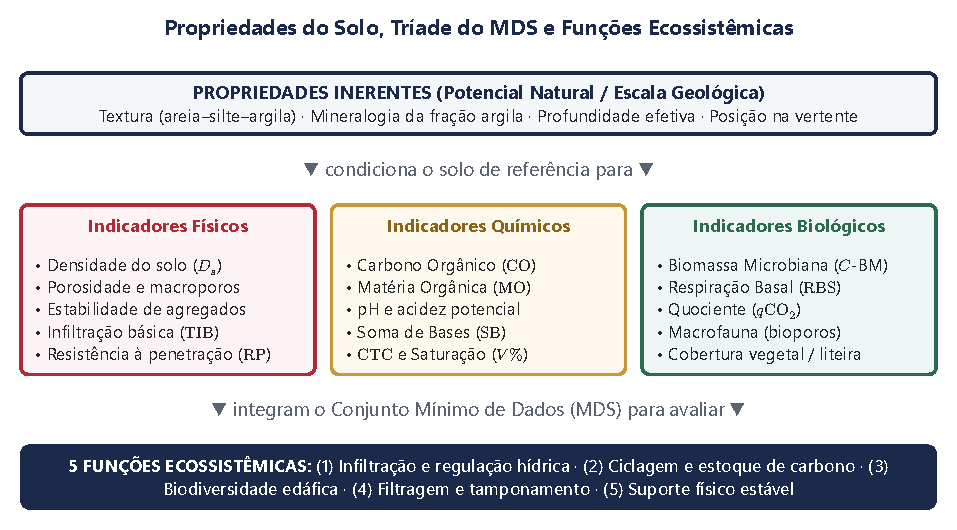
\includegraphics[width=0.92\textwidth]{figures/fig_cap11_triade_mds_funcoes.pdf}
  \caption{Relação entre propriedades inerentes do solo, tríade de indicadores dinâmicos do Conjunto Mínimo de Dados (MDS) e as cinco funções ecossistêmicas avaliadas.}
  \label{fig:triade_mds_funcoes}
\end{figure}

\section{Indicadores Físicos, Químicos e Biológicos do MDS}

\subsection{Indicadores Físicos (Arquitetura Porosa e Fluxo Hídrico)}

Os atributos físicos governam a circulação de água, ar e raízes no perfil edáfico e respondem rapidamente à degradação mecânica observada em pastagens sobrepastoreadas, áreas agrícolas convencionais e acessos de obras civis ou parques eólicos. A \textbf{densidade do solo ($D_s$)} mede a massa de solo seco contida em um volume conhecido de solo estruturado. Para preservar os poros originais sem esmagá-los, coleta-se uma amostra indeformada cravando um cilindro metálico de volume conhecido $V_t$ (anel de Kopecky) no perfil, levando-o à estufa a $105\,^\circ\text{C}$ até massa constante ($m_s$). Quanto maior a compactação imposta pelo tráfego ou pisoteio, mais partículas sólidas são comprimidas no mesmo volume e maior fica $D_s$. Solos minerais conservados exibem tipicamente valores entre $1{,}00$ e $1{,}35\text{ g}\cdot\text{cm}^{-3}$, ao passo que leituras acima de $1{,}55$--$1{,}65\text{ g}\cdot\text{cm}^{-3}$ em solos de textura média a argilosa costumam impor restrição severa ao crescimento radicular.

Para compreender o efeito real dessa compactação sobre a água e o ar, analisa-se a \textbf{porosidade total ($P_t$)} em conjunto com a separação entre \textbf{macroporosidade e microporosidade} (Figura~\ref{fig:porosidade_compactacao}). Na mesa de tensão a $6\text{ kPa}$, drenam-se os \textbf{macroporos} ($> 50\,\mu\text{m}$), responsáveis pela aeração das raízes e pela drenagem rápida da água gravitacional, restando retida a água dos \textbf{microporos} ($< 50\,\mu\text{m}$), que armazenam umidade disponível às plantas. Quando o solo sofre compressão mecânica, os macroporos colapsam primeiro, e valores de macroporosidade inferiores a $10\%$ do volume total tornam-se críticos para a oxigenação radicular.

\begin{figure}[H]
  \centering
  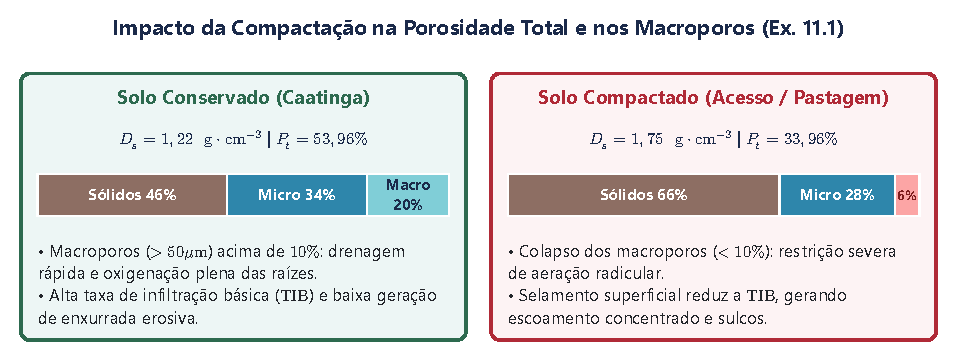
\includegraphics[width=0.92\textwidth]{figures/fig_cap11_porosidade_compactacao.pdf}
  \caption{Impacto da compactação na proporção volumétrica entre sólidos, microporos e macroporos, comparando Caatinga conservada e acesso compactado.}
  \label{fig:porosidade_compactacao}
\end{figure}

A integridade dessa arquitetura porosa depende da \textbf{estabilidade de agregados em água}, medida pelo Diâmetro Médio Ponderado (DMP) após peneiramento úmido. Agregados estáveis resistem ao impacto das gotas de chuva (\textit{splash}), prevenindo o selamento superficial. Quando o selamento ocorre ou os macroporos diminuem, cai abruptamente a \textbf{Taxa de Infiltração Básica ($TIB$)}, medida em campo com infiltrômetro de anéis concêntricos ($\text{mm}\cdot\text{h}^{-1}$), convertendo chuvas moderadas em escoamento superficial concentrado e sulcos erosivos (Figura~\ref{fig:solo_compactado_sulco}). Complementando essa leitura hidráulica, a \textbf{resistência do solo à penetração ($RP$)}, medida com penetrômetro ($\text{MPa}$), avalia o impedimento mecânico às raízes; na capacidade de campo, valores acima de $2{,}0$--$2{,}5\text{ MPa}$ restringem o alongamento radicular.

\begin{figure}[H]
  \centering
  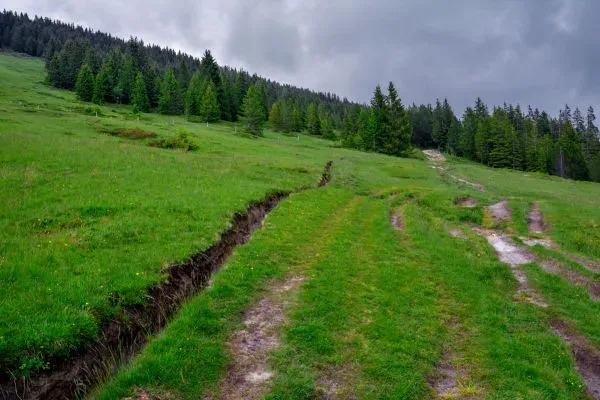
\includegraphics[width=0.78\textwidth]{figures/foto_estrada_sulco_erosivo.jpg}
  \caption{Superfície de solo compactado em acesso rural com selamento superficial, perda de macroporosidade e formação de sulco erosivo por escoamento superficial concentrado. Fonte: acervo didático da disciplina.}
  \label{fig:solo_compactado_sulco}
\end{figure}

As expressões físicas abaixo permitem quantificar densidade, porosidade total e frações porosas a partir do anel saturado ($m_{\text{sat}}$), drenado a $6\text{ kPa}$ ($m_{6\text{kPa}}$) e seco em estufa ($m_s$), com $\rho_{\text{água}} = 1{,}0\text{ g}\cdot\text{cm}^{-3}$:
\[
D_s = \frac{m_s}{V_t} \quad (\text{g}\cdot\text{cm}^{-3}) \qquad\qquad P_t = \left(1 - \frac{D_s}{D_p}\right) \times 100\%
\]
\[
P_{\text{micro}} = \frac{m_{6\text{kPa}} - m_s}{\rho_{\text{água}} \cdot V_t}\times 100\% \qquad\qquad P_{\text{macro}} = \frac{m_{\text{sat}} - m_{6\text{kPa}}}{\rho_{\text{água}} \cdot V_t}\times 100\%
\]

O Exemplo 11.1 aplica diretamente as relações de densidade e porosidade total aos dados representados na Figura~\ref{fig:porosidade_compactacao}.

\begin{boxExemplo}{11.1 (Básico)}{Cálculo de Densidade do Solo e Porosidade Total em Anel Volumétrico}
\passoEnunciado{Durante uma campanha prática da disciplina CHF662, foram coletadas amostras indeformadas ($0$--$10\text{ cm}$) utilizando anéis de Kopecky de $100\text{ cm}^3$ em um fragmento de Caatinga conservada e na borda compactada de um acesso de parque eólico ($D_p = 2{,}65\text{ g}\cdot\text{cm}^{-3}$).}
\passoDados{Volume $V_t = 100\text{ cm}^3$; massa seca na Caatinga $m_{s,1} = 122\text{ g}$; massa seca no acesso compactado $m_{s,2} = 175\text{ g}$.}
\passoPedido{Calcular a densidade do solo ($D_s$) e a porosidade total ($P_t$) em ambos os pontos e interpretar o contraste físico.}
\passoMetodo{Aplicação direta das expressões $D_s = m_s / V_t$ e $P_t = (1 - D_s / D_p)\times 100\%$.}
\passoContas{
\[
D_{s,1} = \frac{122}{100} = 1{,}22\text{ g}\cdot\text{cm}^{-3} \quad\Rightarrow\quad P_{t,1} = \left(1 - \frac{1{,}22}{2{,}65}\right)\times 100\% = 53{,}96\%
\]
\[
D_{s,2} = \frac{175}{100} = 1{,}75\text{ g}\cdot\text{cm}^{-3} \quad\Rightarrow\quad P_{t,2} = \left(1 - \frac{1{,}75}{2{,}65}\right)\times 100\% = 33{,}96\%
\]
Diferença: $P_{t,2} - P_{t,1} = -20{,}00$ pontos percentuais (perda relativa de $37{,}1\%$ do espaço poroso).}
\passoResposta{Caatinga conservada: $D_s = 1{,}22\text{ g}\cdot\text{cm}^{-3}$ e $P_t = 53{,}96\%$. Acesso compactado: $D_s = 1{,}75\text{ g}\cdot\text{cm}^{-3}$ e $P_t = 33{,}96\%$.}
\passoVerificacao{A compactação aumentou $D_s$ em $0{,}53\text{ g}\cdot\text{cm}^{-3}$ e eliminou $20$ pontos percentuais de porosidade, colapsando prioritariamente os macroporos de drenagem rápida.}
\end{boxExemplo}

Quando o diagnóstico físico inclui medições em mesa de tensão, quantifica-se separadamente quanto dessa porosidade total permanece disponível para aeração radicular, conforme mostra o Exemplo 11.4.

\begin{boxExemplo}{11.4 (Avançado)}{Separação de Macro e Microporosidade em Mesa de Tensão}
\passoEnunciado{Uma amostra indeformada de solo ($V_t = 100\text{ cm}^3$) proveniente de uma área em recuperação com bioengenharia foi saturada por capilaridade, submetida à tensão de $6\text{ kPa}$ em mesa de tensão e, finalmente, seca em estufa a $105\,^\circ\text{C}$.}
\passoDados{$V_t = 100\text{ cm}^3$; $\rho_{\text{água}} = 1{,}0\text{ g}\cdot\text{cm}^{-3}$. Massas (descontada a tara): $m_{\text{sat}} = 174\text{ g}$; $m_{6\text{kPa}} = 158\text{ g}$; $m_s = 128\text{ g}$.}
\passoPedido{Determinar $P_t^{\text{sat}}$, $P_{\text{micro}}$ e $P_{\text{macro}}$, avaliando se há restrição de aeração radicular.}
\passoMetodo{Cálculo dos volumes de água retidos em cada estado energético divididos pelo volume do anel.}
\passoContas{
\begin{align*}
P_t^{\text{sat}} &= \frac{174 - 128}{100}\times 100\% = 46{,}0\% \\
P_{\text{micro}} &= \frac{158 - 128}{100}\times 100\% = 30{,}0\% \qquad P_{\text{macro}} = \frac{174 - 158}{100}\times 100\% = 16{,}0\%
\end{align*}
Conferência aditiva: $P_{\text{micro}} + P_{\text{macro}} = 30{,}0\% + 16{,}0\% = 46{,}0\% = P_t^{\text{sat}}$.}
\passoResposta{$P_t^{\text{sat}} = 46{,}0\%$, $P_{\text{micro}} = 30{,}0\%$ e $P_{\text{macro}} = 16{,}0\%$, superando o limiar mínimo de $10\%$ sem restrição crítica à aeração.}
\passoVerificacao{A proporção de cerca de um terço de macroporos e dois terços de microporos aproxima-se do equilíbrio físico desejável para armazenamento hídrico aliado à drenagem interna.}
\end{boxExemplo}

Na interpretação de campo dos indicadores físicos, dois equívocos metodológicos comprometem os laudos de degradação: comparar solos de texturas distintas sem referência local e medir resistência à penetração sem registrar a umidade.

\begin{boxErro}[Erro 1: Comparar Áreas em Solos de Texturas Distintas Sem Referência Local]
\textbf{Equívoco frequente:} Classificar um Neossolo Quartzarênico arenoso ($D_s = 1{,}45\text{ g}\cdot\text{cm}^{-3}$) como degradado comparando-o a um Latossolo argiloso conservado ($D_s = 1{,}05\text{ g}\cdot\text{cm}^{-3}$).\par
\textbf{Correção técnica:} Solos arenosos possuem naturalmente maior densidade e menor $CTC$ do que solos argilosos bem estruturados. A área de referência sob vegetação nativa deve pertencer à \textbf{mesma classe de solo, textura e posição geomorfológica} da área diagnosticada.
\end{boxErro}

No Semiárido, a sazonalidade hídrica amplia drasticamente a coesão aparente do solo seco, exigindo cuidado adicional nas leituras de penetrômetro.

\begin{boxErro}[Erro 2: Avaliar Resistência à Penetração ($RP$) Sem Registrar a Umidade do Solo]
\textbf{Equívoco frequente:} Medir $RP$ na estação seca no Semiárido, obter valores acima de $4{,}0\text{ MPa}$ e diagnosticar compactação antrópica irreversível.\par
\textbf{Correção técnica:} A resistência mecânica à penetração aumenta exponencialmente à medida que o solo seca, devido à coesão entre partículas e à sucção matricial. Leituras de penetrômetro só são comparáveis quando realizadas sob umidade controlada (próxima à capacidade de campo) ou acompanhadas do teor gravimétrico de umidade.
\end{boxErro}

\subsection{Indicadores Químicos (Matéria Orgânica, Acidez e Troca Catiônica)}

Os atributos químicos determinam a disponibilidade de nutrientes, o poder tampão e a estabilidade coloidal do solo. Nesse compartimento, a \textbf{Matéria Orgânica ($MO$)} e o \textbf{Carbono Orgânico Total ($CO$)} integram física, química e biologia porque cimentam agregados, elevam a retenção de água e fornecem a maior parte das cargas negativas responsáveis pela $CTC$ em solos tropicais intemperizados. Como os métodos laboratoriais (Walkley--Black ou combustão seca) quantificam diretamente o carbono orgânico ($CO$), estima-se a matéria orgânica multiplicando $CO$ pelo \textbf{fator de van Bemmelen ($1{,}724$)}, baseado na convenção de que a matéria orgânica humificada contém aproximadamente $58\%$ de carbono em massa ($1 / 0{,}58 \approx 1{,}724$). As equações químicas abaixo permitem converter $CO$ em $MO$ e calcular o estoque de carbono ($EC$, em $\text{Mg C}\cdot\text{ha}^{-1}$) na camada de espessura $h_{\text{m}}$ (utilizando $1\text{ g}\cdot\text{cm}^{-3} = 1\text{ Mg}\cdot\text{m}^{-3}$):
\[
CO = \frac{MO}{1{,}724} \quad \Longleftrightarrow \quad MO = CO \times 1{,}724 \qquad\qquad EC = \left(\frac{CO_{\text{g/kg}}}{1000}\right) \cdot D_s \cdot (10.000 \cdot h_{\text{m}})
\]

O Exemplo 11.2 demonstra como padronizar laudos expressos em grandezas distintas e quantificar a perda de carbono por hectare.

\begin{boxExemplo}{11.2 (Básico/Intermediário)}{Fator de van Bemmelen e Estoque de Carbono na Camada 0--20 cm}
\passoEnunciado{Um laudo laboratorial reportou carbono orgânico total de $18{,}0\text{ g}\cdot\text{kg}^{-1}$ em um solo sob Caatinga preservada (Área A, $D_s = 1{,}25\text{ g}\cdot\text{cm}^{-3}$). Em uma pastagem degradada adjacente no mesmo solo (Área B, $D_s = 1{,}60\text{ g}\cdot\text{cm}^{-3}$), outro laboratório expressou o resultado em matéria orgânica total, $MO = 12{,}068\text{ g}\cdot\text{kg}^{-1}$.}
\passoDados{Camada $h = 0{,}20\text{ m}$. Área A: $CO_A = 18{,}0\text{ g}\cdot\text{kg}^{-1}$, $D_{s,A} = 1{,}25$. Área B: $MO_B = 12{,}068\text{ g}\cdot\text{kg}^{-1}$, $D_{s,B} = 1{,}60$. Fator de van Bemmelen: $1{,}724$.}
\passoPedido{Calcular o teor de $MO$ na Área A, o teor de $CO$ na Área B, o estoque de carbono ($EC$, em $\text{Mg C}\cdot\text{ha}^{-1}$) nas duas áreas e a perda líquida de carbono.}
\passoMetodo{Conversão via fator de van Bemmelen ($MO = 1{,}724 \cdot CO$) e cálculo da massa de solo por hectare na camada de $0{,}20\text{ m}$.}
\passoContas{
\[
MO_A = 18{,}0 \times 1{,}724 = 31{,}032\text{ g}\cdot\text{kg}^{-1} \quad (3{,}10\%) \qquad\qquad CO_B = \frac{12{,}068}{1{,}724} = 7{,}00\text{ g}\cdot\text{kg}^{-1} \quad (0{,}70\%)
\]
Volume em $1\text{ ha}$ ($0{,}20\text{ m}$): $V_{\text{ha}} = 2.000\text{ m}^3\cdot\text{ha}^{-1}$.
Área A: massa $= 2.000 \times 1{,}25 = 2.500\text{ Mg}\cdot\text{ha}^{-1} \Rightarrow EC_A = 2.500 \times 0{,}018 = 45{,}00\text{ Mg C}\cdot\text{ha}^{-1}$.
Área B: massa $= 2.000 \times 1{,}60 = 3.200\text{ Mg}\cdot\text{ha}^{-1} \Rightarrow EC_B = 3.200 \times 0{,}007 = 22{,}40\text{ Mg C}\cdot\text{ha}^{-1}$.
Perda líquida: $\Delta EC = 45{,}00 - 22{,}40 = 22{,}60\text{ Mg C}\cdot\text{ha}^{-1}$ ($-50{,}2\%$).}
\passoResposta{Área A: $MO = 31{,}032\text{ g}\cdot\text{kg}^{-1}$ e $EC = 45{,}00\text{ Mg C}\cdot\text{ha}^{-1}$. Área B: $CO = 7{,}00\text{ g}\cdot\text{kg}^{-1}$ e $EC = 22{,}40\text{ Mg C}\cdot\text{ha}^{-1}$. Perda líquida de $22{,}60\text{ Mg C}\cdot\text{ha}^{-1}$.}
\passoVerificacao{Mesmo com maior massa de solo em $20\text{ cm}$ na Área B devido à compactação ($3.200$ vs. $2.500\text{ Mg}$), a perda já ultrapassa metade do estoque original.}
\end{boxExemplo}

Na comparação entre laudos laboratoriais diferentes, um erro frequente decorre da troca direta entre carbono orgânico e matéria orgânica sem aplicar o fator de conversão.

\begin{boxErro}[Erro 3: Confundir Carbono Orgânico ($CO$) com Matéria Orgânica ($MO$)]
\textbf{Equívoco frequente:} Comparar diretamente um laudo expresso em $CO$ ($\text{g}\cdot\text{kg}^{-1}$) com outro expresso em $MO$ ($\text{g}\cdot\text{kg}^{-1}$) sem conversão prévia.\par
\textbf{Correção técnica:} A matéria orgânica contém carbono, oxigênio, hidrogênio e nitrogênio; portanto, $MO$ é sempre numericamente maior que $CO$ ($MO = 1{,}724 \times CO$). Padronize todas as amostras na mesma grandeza antes de comparar resultados ou calcular estoques de carbono.
\end{boxErro}

O \textbf{potencial hidrogeniônico (pH)} controla a solubilidade de nutrientes e a toxicidade do alumínio trocável ($Al^{3+}$) abaixo de pH $5{,}5$. No Semiárido Baiano, Luvissolos e Neossolos pouco intemperizados tendem a apresentar pH levemente ácido a neutro ($6{,}0$--$7{,}2$), enquanto Latossolos profundos de tabuleiros costumam ser mais ácidos ($4{,}5$--$5{,}5$). Associando a \textbf{Soma de Bases ($SB$)} à acidez potencial ($H^+ + Al^{3+}$), obtém-se a $CTC$ a pH $7{,}0$ e a \textbf{Saturação por Bases ($V\%$)}:
\[
SB = Ca^{2+} + Mg^{2+} + K^+ + Na^+ \qquad CTC = SB + (H^+ + Al^{3+}) \qquad V\% = \frac{SB}{CTC}\times 100\%
\]
Solos com $V\% \ge 50\%$ são classificados como \textbf{eutróficos} (alta fertilidade natural), ao passo que solos com $V\% < 50\%$ são \textbf{distróficos} (baixa fertilidade natural). O Exemplo 11.3 contrasta essas duas classes pedológicas na Bahia.

\begin{boxExemplo}{11.3 (Intermediário)}{Diagnóstico Químico: Soma de Bases, CTC e Saturação por Bases ($V\%$)}
\passoEnunciado{Compare os laudos químicos de rotina (camada $0$--$20\text{ cm}$) de dois solos baianos: Solo 1 (Luvissolo Crômico sob Caatinga no Semiárido) e Solo 2 (Latossolo Amarelo sob pastagem degradada nos Tabuleiros Costeiros).}
\passoDados{Valores em $\text{cmol}_c\cdot\text{dm}^{-3}$. Solo 1: $Ca^{2+} = 5{,}40$; $Mg^{2+} = 2{,}60$; $K^+ = 0{,}45$; $Na^+ = 0{,}15$; $H^+ + Al^{3+} = 2{,}40$. Solo 2: $Ca^{2+} = 1{,}20$; $Mg^{2+} = 0{,}60$; $K^+ = 0{,}15$; $Na^+ = 0{,}05$; $H^+ + Al^{3+} = 4{,}00$.}
\passoPedido{Calcular $SB$, $CTC$ a pH $7{,}0$ e $V\%$ para os dois solos e classificá-los quanto ao caráter eutrófico ou distrófico.}
\passoMetodo{Aplicação das equações aditivas de $SB$ e $CTC$ e cálculo da razão percentual $V\% = (SB / CTC)\times 100\%$.}
\passoContas{
\begin{align*}
SB_1 &= 8{,}60\text{ cmol}_c\cdot\text{dm}^{-3} \qquad & CTC_1 &= 8{,}60 + 2{,}40 = 11{,}00\text{ cmol}_c\cdot\text{dm}^{-3} \\
V\%_1 &= \frac{8{,}60}{11{,}00}\times 100\% = 78{,}18\% & & \\[4pt]
SB_2 &= 2{,}00\text{ cmol}_c\cdot\text{dm}^{-3} \qquad & CTC_2 &= 2{,}00 + 4{,}00 = 6{,}00\text{ cmol}_c\cdot\text{dm}^{-3} \\
V\%_2 &= \frac{2{,}00}{6{,}00}\times 100\% = 33{,}33\% & &
\end{align*}}
\passoResposta{Solo 1: $SB = 8{,}60$, $CTC = 11{,}00\text{ cmol}_c\cdot\text{dm}^{-3}$ e $V\% = 78{,}18\%$ (eutrófico). Solo 2: $SB = 2{,}00$, $CTC = 6{,}00\text{ cmol}_c\cdot\text{dm}^{-3}$ e $V\% = 33{,}33\%$ (distrófico).}
\passoVerificacao{No Semiárido, a menor lixiviação preserva bases trocáveis, enquanto nos ambientes úmidos a intensa lixiviação combinada à perda de matéria orgânica reduz $SB$, $CTC$ e $V\%$.}
\end{boxExemplo}

\subsection{Indicadores Biológicos (Motor Vivo da Funcionalidade Edáfica)}

Os indicadores biológicos costumam responder às perturbações iniciais e às ações de recuperação antes que os estoques totais de carbono ou a densidade exibam alterações mensuráveis. O \textbf{Carbono da Biomassa Microbiana ($C\text{-BM}$)} representa a fração viva da matéria orgânica (fungos, bactérias e actinomicetos, geralmente entre $1\%$ e $4\%$ do $CO$ total) e reage em poucos meses ao manejo. Interpretado junto à \textbf{Respiração Basal do Solo ($RBS$)}, que mede a liberação de $\text{CO}_2$ pela atividade metabólica, o quociente metabólico ($q\text{CO}_2 = RBS / C\text{-BM}$) funciona como termômetro de estresse ecológico: valores elevados indicam que os microrganismos gastam mais energia na manutenção celular do que no crescimento. Completa esse eixo a \textbf{fauna edáfica e a cobertura vegetal}, pois minhocas, térmitas e formigas constroem bioporos enquanto a serapilheira amortece a temperatura superficial. Em pastagens degradadas sem cobertura vegetal, a atividade biológica entra em colapso e o solo exposto evolui rapidamente para ravinas (Figura~\ref{fig:pastagem_ravinas}).

\begin{figure}[H]
  \centering
  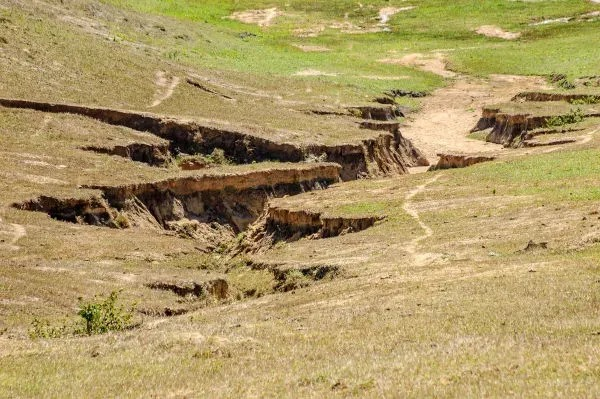
\includegraphics[width=0.78\textwidth]{figures/foto_pastagem_ravinas.jpg}
  \caption{Pastagem degradada com perda de cobertura vegetal, exposição do horizonte mineral e evolução de ravinas em vertente. Fonte: acervo didático da disciplina.}
  \label{fig:pastagem_ravinas}
\end{figure}

\section{Normalização Linear, Cálculo do IQS e Visualização Multivariada}

Como cada indicador possui unidade distinta ($\text{g}\cdot\text{kg}^{-1}$, $\text{mm}\cdot\text{h}^{-1}$, $\text{g}\cdot\text{cm}^{-3}$), converte-se cada valor bruto $x_i$ em uma nota adimensional $S_i \in [0, 1]$ para viabilizar a agregação matemática (Figura~\ref{fig:curvas_normalizacao}). Para atributos cuja elevação favorece a funcionalidade edáfica (\textbf{``quanto maior melhor''}, como $MO$, $P_t$, $TIB$ e $DMP$), aplica-se $S_i = \min\!\left(1;\; \dfrac{x_i}{x_{\text{ref}}}\right)$, travando a nota máxima em $1{,}0$. Para atributos cujo aumento indica restrição física (\textbf{``quanto menor melhor''}, como $D_s$ e $RP$), inverte-se a razão, $S_i = \min\!\left(1;\; \dfrac{x_{\text{ref}}}{x_i}\right)$.

\begin{figure}[H]
  \centering
  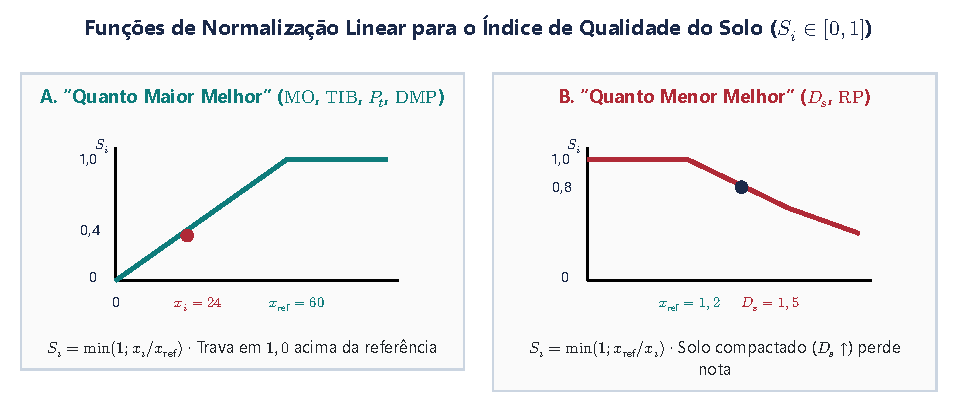
\includegraphics[width=0.92\textwidth]{figures/fig_cap11_curvas_normalizacao.pdf}
  \caption{Curvas das funções de normalização linear para indicadores ``quanto maior melhor'' (A) e ``quanto menor melhor'' (B), mostrando os pontos de referência e o comportamento fora da faixa ótima.}
  \label{fig:curvas_normalizacao}
\end{figure}

Agregando as pontuações $S_i$, calcula-se o Índice de Qualidade do Solo simples ou ponderado:
\[
\text{IQS}_{\text{simples}} = \frac{1}{n}\sum_{i=1}^{n} S_i \qquad \text{ou} \qquad \text{IQS}_{\text{ponderado}} = \sum_{i=1}^{n} w_i \, S_i \quad \left(\text{com } \sum_{i=1}^{n} w_i = 1\right)
\]

A integração dessas notas normalizadas em um \textbf{gráfico radar} (Figura~\ref{fig:qualidade_solo_radar}) preserva simultaneamente a visão global (área do polígono proporcional ao IQS) e o diagnóstico individual de cada gargalo (eixos recolhidos próximo ao centro).

\begin{figure}[H]
  \centering
  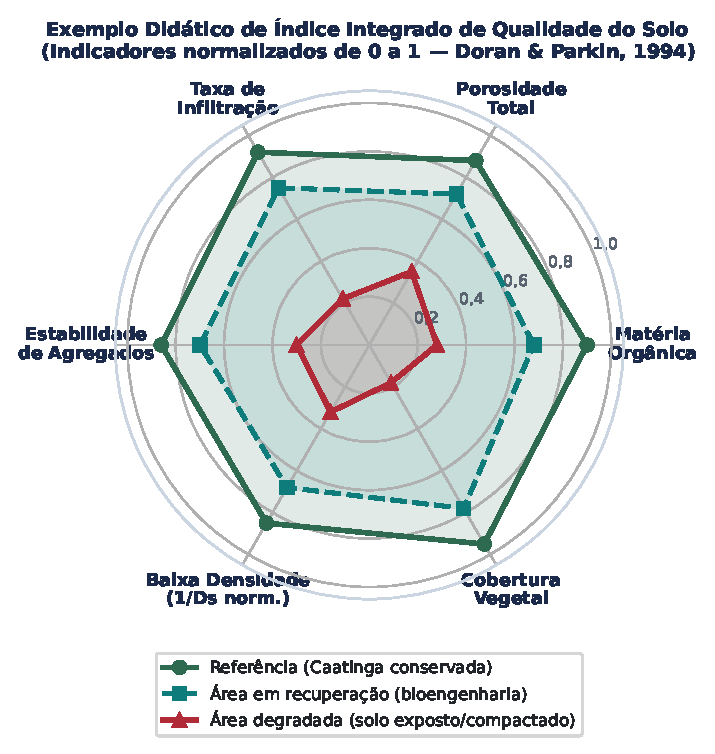
\includegraphics[width=0.80\textwidth]{figures/fig09_qualidade_solo_radar.pdf}
  \caption{Comparação multivariada de seis indicadores normalizados de qualidade do solo ($0$ a $1$) entre área de referência sob Caatinga conservada, área em recuperação com técnicas de bioengenharia e área degradada com solo exposto e compactado.}
  \label{fig:qualidade_solo_radar}
\end{figure}

Observando os cenários plotados (Figura~\ref{fig:qualidade_solo_radar}), a \textbf{área de referência sob Caatinga conservada} apresenta escores entre $0{,}85$ e $0{,}95$, resultando em $\text{IQS} = (0{,}90+0{,}88+0{,}92+0{,}86+0{,}85+0{,}95)/6 = \mathbf{0{,}893}$ (qualidade muito alta). A \textbf{área em recuperação com bioengenharia} alcança escores entre $0{,}68$ e $0{,}78$, com $\text{IQS} = \mathbf{0{,}718}$ (trajetória ascendente, com matéria orgânica e densidade ainda em consolidação). Já a \textbf{área degradada} exibe escores colapsados entre $0{,}18$ (cobertura vegetal) e $0{,}35$ (porosidade total), produzindo $\text{IQS} = \mathbf{0{,}275}$ e demandando intervenção prioritária na cobertura superficial e descompactação biológica.

\etapa{4}{Síntese Integrada do Índice de Qualidade do Solo}

O Exemplo 11.5 consolida a passagem completa das medições brutas em campo e laboratório até o cálculo dos índices simples e ponderado.

\begin{boxExemplo}{11.5 (Avançado)}{Normalização Linear e Cálculo Completo do Índice de Qualidade do Solo (IQS)}
\passoEnunciado{Para o Trabalho Prático Final, um grupo selecionou quatro indicadores para avaliar uma encosta submetida à recuperação ambiental frente a uma mata de referência no mesmo solo.}
\passoDados{$MO$ (``maior melhor''): avaliada $= 16{,}0\text{ g}\cdot\text{kg}^{-1}$, ref. $= 32{,}0$, $w_1 = 0{,}30$; $TIB$ (``maior melhor''): avaliada $= 24{,}0\text{ mm}\cdot\text{h}^{-1}$, ref. $= 60{,}0$, $w_2 = 0{,}30$; $D_s$ (``menor melhor''): avaliada $= 1{,}50\text{ g}\cdot\text{cm}^{-3}$, ref. $= 1{,}20$, $w_3 = 0{,}20$; $DMP$ (``maior melhor''): avaliada $= 1{,}25\text{ mm}$, ref. $= 2{,}50$, $w_4 = 0{,}20$.}
\passoPedido{Calcular a pontuação normalizada $S_i$ de cada indicador, o $\text{IQS}_{\text{simples}}$ e o $\text{IQS}_{\text{ponderado}}$, indicando o gargalo prioritário.}
\passoMetodo{Normalização linear conforme as curvas da Figura~\ref{fig:curvas_normalizacao} seguida das médias aritmética e ponderada.}
\passoContas{
\begin{align*}
  S_{MO} &= \frac{16{,}0}{32{,}0} = 0{,}50 \qquad & S_{TIB} &= \frac{24{,}0}{60{,}0} = 0{,}40 \\
  S_{D_s} &= \frac{1{,}20}{1{,}50} = 0{,}80 \;\text{(invertida)} \qquad & S_{DMP} &= \frac{1{,}25}{2{,}50} = 0{,}50
\end{align*}
\begin{align*}
  \text{IQS}_{\text{simples}} &= \frac{0{,}50 + 0{,}40 + 0{,}80 + 0{,}50}{4} = 0{,}550 \\
  \text{IQS}_{\text{ponderado}} &= (0{,}30 \times 0{,}50) + (0{,}30 \times 0{,}40) + (0{,}20 \times 0{,}80) + (0{,}20 \times 0{,}50) = 0{,}530
\end{align*}}
\passoResposta{Pontuações: $S_{MO}=0{,}50$, $S_{TIB}=0{,}40$, $S_{D_s}=0{,}80$, $S_{DMP}=0{,}50$. $\text{IQS}_{\text{simples}} = 0{,}550$ e $\text{IQS}_{\text{ponderado}} = 0{,}530$ (qualidade moderada). O gargalo prioritário é a taxa de infiltração básica ($S_{TIB} = 0{,}40$).}
\passoVerificacao{O $\text{IQS}_{\text{ponderado}}$ ($0{,}530$) ficou abaixo do simples ($0{,}550$) porque os maiores pesos ($0{,}30$) recaíram sobre infiltração e matéria orgânica, orientando ações focadas em cobertura morta e aporte orgânico.}
\end{boxExemplo}

\etapa{5}{Cuidado Final na Normalização e Materiais Audiovisuais de Apoio}

Ao calcular o IQS em planilhas eletrônicas, verifique sempre o sentido da função de normalização antes de gerar o gráfico radar, evitando o erro algébrico descrito a seguir.

\begin{boxErro}[Erro 4: Usar a Fórmula ``Quanto Maior Melhor'' para Densidade do Solo ($D_s$)]
\textbf{Equívoco frequente:} Normalizar $D_s$ dividindo o valor da área degradada ($1{,}75$) pelo da referência ($1{,}20$), obtendo escore superior a $1{,}0$ e premiando um solo severamente compactado.\par
\textbf{Correção técnica:} Para densidade do solo e resistência à penetração, valores maiores indicam pior qualidade física. Aplica-se obrigatoriamente a função \textbf{``quanto menor melhor''}: $S_{D_s} = \min(1;\; D_{s,\text{ref}} / D_{s,\text{avaliado}})$.
\end{boxErro}

Para consolidar a visualização dos indicadores físicos, químicos e biológicos em campo e laboratório, consulte os vídeos selecionados na página da disciplina: \textit{Análise da Saúde do Solo} (\url{https://www.youtube.com/watch?v=D8jI-ltuzVI}, cerca de 7 min, integrando matéria orgânica, densidade, porosidade e biologia edáfica), \textit{Saúde do Solo: Qualidade Biológica} (\url{https://www.youtube.com/watch?v=WHh50dAM4as}, focado em indicadores biológicos tropicais) e \textit{Degradação dos Solos} (\url{https://www.youtube.com/watch?v=QujBcIOl3qQ}, cerca de 17 min, ilustrando lixiviação, erosão, laterização e salinização).

\etapa{6}{Exercícios de Fixação}

\subsection*{Nível Básico (Conceitos de Funcionalidade Edáfica e MDS)}

\begin{enumerate}[leftmargin=1.8em, itemsep=6pt]
  \item Explique por que o conceito contemporâneo de \textbf{Qualidade do Solo} (Doran; Parkin, 1994; Karlen et al., 1997) é mais abrangente do que a noção tradicional de fertilidade química agrícola.
  \espacoResolucao[1.8cm]

  \item Diferencie \textbf{propriedades inerentes} de \textbf{propriedades dinâmicas} do solo, citando dois exemplos de cada grupo.
  \espacoResolucao[1.8cm]

  \item Qual é o significado físico e matemático do \textbf{fator de van Bemmelen ($1{,}724$)} na conversão entre carbono orgânico total ($CO$) e matéria orgânica ($MO$)?
  \espacoResolucao[1.8cm]

  \item Por que a \textbf{macroporosidade} é mais sensível à compactação do solo do que a porosidade total ($P_t$), e qual é o seu limiar crítico de aeração radicular?
  \espacoResolucao[1.8cm]

  \item Explique por que o \textbf{Carbono da Biomassa Microbiana ($C\text{-BM}$)} e o quociente metabólico ($q\text{CO}_2$) são indicadores precoces valiosos no monitoramento de áreas degradadas em recuperação.
  \espacoResolucao[1.8cm]
\end{enumerate}

\subsection*{Nível Intermediário (Cálculos Físicos, Químicos e IQS)}

\begin{enumerate}[leftmargin=1.8em, itemsep=6pt, resume]
  \item Uma amostra indeformada coletada em anel volumétrico de $100\text{ cm}^3$ apresentou massa de solo seco em estufa de $159\text{ g}$. Considerando densidade de partículas $D_p = 2{,}65\text{ g}\cdot\text{cm}^{-3}$, calcule a densidade do solo ($D_s$) e a porosidade total ($P_t$).
  \espacoResolucao[2.2cm]

  \item Um solo sob Caatinga em regeneração apresentou teor de matéria orgânica $MO = 25{,}86\text{ g}\cdot\text{kg}^{-1}$ e densidade do solo $D_s = 1{,}30\text{ g}\cdot\text{cm}^{-3}$ na camada $0$--$20\text{ cm}$. Calcule o teor de carbono orgânico total ($CO$, em $\text{g}\cdot\text{kg}^{-1}$) usando o fator de van Bemmelen e o estoque de carbono ($EC$, em $\text{Mg C}\cdot\text{ha}^{-1}$) nessa camada.
  \espacoResolucao[2.2cm]

  \item Um laudo químico forneceu os seguintes valores (em $\text{cmol}_c\cdot\text{dm}^{-3}$): $Ca^{2+} = 4{,}20$; $Mg^{2+} = 1{,}80$; $K^+ = 0{,}30$; $Na^+ = 0{,}10$; e $H^+ + Al^{3+} = 3{,}60$. Calcule $SB$, $CTC$ e $V\%$, classificando o solo como eutrófico ou distrófico.
  \espacoResolucao[2.2cm]

  \item Em ensaio de mesa de tensão com anel de $100\text{ cm}^3$ ($\rho_{\text{água}} = 1{,}0\text{ g}\cdot\text{cm}^{-3}$), obtiveram-se as massas (sem a tara do anel): $m_{\text{sat}} = 165\text{ g}$, $m_{6\text{kPa}} = 157\text{ g}$ e $m_s = 130\text{ g}$. Calcule $P_t^{\text{sat}}$, $P_{\text{micro}}$ e $P_{\text{macro}}$, indicando se há risco físico à aeração das raízes.
  \espacoResolucao[2.2cm]

  \item Calcule o $\text{IQS}_{\text{simples}}$ de uma parcela degradada a partir dos três indicadores abaixo e identifique o indicador de menor desempenho:
  \begin{itemize}[leftmargin=1.4em, itemsep=1pt]
    \item $MO$ (maior melhor): parcela $= 20\text{ g}\cdot\text{kg}^{-1}$; referência $= 40\text{ g}\cdot\text{kg}^{-1}$.
    \item $TIB$ (maior melhor): parcela $= 36\text{ mm}\cdot\text{h}^{-1}$; referência $= 60\text{ mm}\cdot\text{h}^{-1}$.
    \item $D_s$ (menor melhor): parcela $= 1{,}60\text{ g}\cdot\text{cm}^{-3}$; referência $= 1{,}20\text{ g}\cdot\text{cm}^{-3}$.
  \end{itemize}
  \espacoResolucao[2.2cm]
\end{enumerate}

\subsection*{Nível Aplicado (Questões Objetivas A--E)}

\begin{enumerate}[leftmargin=1.8em, itemsep=6pt, resume]
  \item A respeito do Conjunto Mínimo de Dados (MDS) para avaliação da qualidade do solo (Doran; Parkin, 1994; Vezzani; Mielniczuk, 2009), assinale a alternativa correta:
  \begin{alternativas}
    \item Deve conter apenas variáveis químicas de rotina, pois atributos físicos e biológicos não se alteram com o manejo da terra.
    \item Deve integrar um número enxuto e representativo de indicadores físicos, químicos e biológicos sensíveis às mudanças de uso da terra.
    \item Exige a medição simultânea de todos os 50 atributos laboratoriais existentes, independentemente de redundância ou custo.
    \item Dispensa a adoção de áreas de referência sob vegetação nativa por utilizar valores absolutos idênticos para qualquer textura de solo.
    \item Restringe-se ao estudo de solos hidromórficos de várzea.
  \end{alternativas}

  \item Um solo mineral com densidade de partículas $D_p = 2{,}65\text{ g}\cdot\text{cm}^{-3}$ e densidade do solo $D_s = 1{,}325\text{ g}\cdot\text{cm}^{-3}$ apresenta porosidade total ($P_t$) exatamente igual a:
  \begin{alternativas}
    \item $25{,}0\%$.
    \item $40{,}0\%$.
    \item $45{,}0\%$.
    \item $50{,}0\%$.
    \item $60{,}0\%$.
  \end{alternativas}

  \item Sobre a normalização de indicadores no cálculo do Índice de Qualidade do Solo (IQS), é correto afirmar que:
  \begin{alternativas}
    \item Indicadores como taxa de infiltração básica e matéria orgânica seguem a função ``quanto menor melhor''.
    \item A normalização converte grandezas com unidades diferentes para uma escala adimensional comum (como $0$ a $1$), possibilitando a agregação matemática.
    \item A densidade do solo deve ser normalizada pela razão $D_{s,\text{avaliado}} / D_{s,\text{referência}}$ para que solos mais compactados recebam notas maiores.
    \item O uso de pesos diferenciados ($w_i$) é proibido em índices de qualidade ambiental.
    \item Um IQS igual a $0{,}25$ indica funcionalidade edáfica superior à da área de referência.
  \end{alternativas}

  \item Se uma amostra de solo apresenta teor de carbono orgânico total $CO = 10{,}0\text{ g}\cdot\text{kg}^{-1}$, o teor estimado de matéria orgânica ($MO$) pelo fator de van Bemmelen ($1{,}724$) é:
  \begin{alternativas}
    \item $5{,}80\text{ g}\cdot\text{kg}^{-1}$.
    \item $10{,}00\text{ g}\cdot\text{kg}^{-1}$.
    \item $15{,}80\text{ g}\cdot\text{kg}^{-1}$.
    \item $17{,}24\text{ g}\cdot\text{kg}^{-1}$.
    \item $27{,}24\text{ g}\cdot\text{kg}^{-1}$.
  \end{alternativas}

  \item Na interpretação do gráfico radar de qualidade do solo (Figura~\ref{fig:qualidade_solo_radar}), uma área degradada que apresenta valores normalizados muito baixos em \textit{cobertura vegetal} ($0{,}18$) e \textit{taxa de infiltração} ($0{,}22$) sinaliza prioritariamente:
  \begin{alternativas}
    \item Alta resiliência física da superfície do solo frente a chuvas intensas.
    \item Predomínio de drenagem profunda com risco nulo de escoamento superficial.
    \item Forte vulnerabilidade ao impacto da gota de chuva, selamento superficial e geração de enxurrada erosiva.
    \item Excesso de matéria orgânica humificada na camada superficial.
    \item Equivalência funcional plena em relação à Caatinga conservada.
  \end{alternativas}
\end{enumerate}

\etapa{7}{Questões no Estilo ENADE e Concursos Ambientais}

\begin{boxDica}[Atenção às Armadilhas em Questões de Solos]
Em provas de Geografia e concursos ambientais, dois detalhes costumam decidir questões: verificar se a tabela fornece \textbf{Carbono Orgânico ($CO$)} ou \textbf{Matéria Orgânica ($MO$)} antes de multiplicar ou dividir por $1{,}724$, e observar o sentido da normalização (``maior melhor'' vs. ``menor melhor'') em indicadores como $D_s$ e $RP$.
\end{boxDica}

\begin{enumerate}[leftmargin=1.8em, itemsep=7pt]
  \item \textbf{[Questão Autoral, Estilo ENADE / Geografia]} Dois talhões localizados sobre a mesma classe de solo no Semiárido Baiano foram avaliados quanto à funcionalidade edáfica. O Talhão X (Caatinga conservada) exibiu $D_s = 1{,}20\text{ g}\cdot\text{cm}^{-3}$, $P_{\text{macro}} = 18\%$, $MO = 30\text{ g}\cdot\text{kg}^{-1}$ e $TIB = 65\text{ mm}\cdot\text{h}^{-1}$. O Talhão Y (área de empréstimo de terra após obra viária) apresentou $D_s = 1{,}72\text{ g}\cdot\text{cm}^{-3}$, $P_{\text{macro}} = 6\%$, $MO = 7\text{ g}\cdot\text{kg}^{-1}$ e $TIB = 9\text{ mm}\cdot\text{h}^{-1}$. Com base nesses resultados, analise as asserções:
  \begin{quote}
    \textbf{I.} O Talhão Y encontra-se fisicamente degradado e sob elevada suscetibilidade ao escoamento superficial concentrado e à erosão hídrica.\\
    \textbf{PORQUE}\\
    \textbf{II.} A perda de matéria orgânica e o colapso da macroporosidade abaixo de $10\%$ comprometem a estabilidade dos agregados e reduzem drasticamente a taxa de infiltração básica do solo.
  \end{quote}
  A respeito dessas asserções, assinale a opção correta:
  \begin{alternativas}
    \item As asserções I e II são proposições verdadeiras, e a II é uma justificativa correta da I.
    \item As asserções I e II são proposições verdadeiras, mas a II não é uma justificativa correta da I.
    \item A asserção I é uma proposição verdadeira, e a II é uma proposição falsa.
    \item A asserção I é uma proposição falsa, e a II é uma proposição verdadeira.
    \item As asserções I e II são proposições falsas.
  \end{alternativas}

  \item \textbf{[Questão Autoral, Estilo Concurso Analista Ambiental]} Em um diagnóstico pedológico para elaboração de PRAD, a análise química da camada superficial de uma área degradada revelou Soma de Bases $SB = 3{,}20\text{ cmol}_c\cdot\text{dm}^{-3}$ e Capacidade de Troca Catiônica a pH $7{,}0$ de $CTC = 8{,}00\text{ cmol}_c\cdot\text{dm}^{-3}$. Com base nesses valores, a saturação por bases ($V\%$) e a classificação química do solo são, respectivamente:
  \begin{alternativas}
    \item $25{,}0\%$, eutrófico.
    \item $40{,}0\%$, distrófico.
    \item $40{,}0\%$, eutrófico.
    \item $60{,}0\%$, distrófico.
    \item $60{,}0\%$, eutrófico.
  \end{alternativas}

  \item \textbf{[Questão Autoral, Estilo Concurso Perito / Geógrafo Ambiental]} Sobre a escolha e o uso de indicadores biológicos na avaliação da qualidade do solo (Vezzani; Mielniczuk, 2009; Karlen et al., 1997), assinale a alternativa \textbf{INCORRETA}:
  \begin{alternativas}
    \item A fauna edáfica (como minhocas, formigas e térmitas) contribui para a formação de bioporos que aumentam a infiltração de água e a aeração do perfil.
    \item O carbono da biomassa microbiana tende a responder mais rapidamente a mudanças de uso da terra do que o estoque total de carbono orgânico.
    \item Valores muito elevados de quociente metabólico ($q\text{CO}_2$) em áreas degradadas podem indicar estresse sobre a comunidade microbiana, que despende maior proporção de carbono em respiração de manutenção.
    \item A cobertura vegetal e a serapilheira modulam a temperatura e a umidade do solo, favorecendo a atividade biológica em ambientes tropicais e semiáridos.
    \item Indicadores biológicos dispensam totalmente a avaliação de densidade do solo e infiltração, pois a presença de micro-organismos elimina a compactação mecânica em poucos dias.
  \end{alternativas}
\end{enumerate}

\clearpage
\etapa{8}{Gabarito Comentado do Capítulo 11}

\begin{boxGabarito}[Resoluções Completas: Exercícios de Fixação (1 a 15)]
\begin{enumerate}[leftmargin=1.6em, itemsep=4pt]
  \item A fertilidade química clássica foca na disponibilidade imediata de nutrientes para produção vegetal. Já a \textbf{Qualidade do Solo} avalia o conjunto das funções ecossistêmicas (regulação hídrica, filtragem de poluentes, estocagem de carbono, sustentação da biodiversidade e resistência à erosão), exigindo integração de atributos físicos, químicos e biológicos.
  \item \textbf{Propriedades inerentes:} dependem dos fatores de formação e variam pouco em escala humana (ex.: textura do solo e mineralogia da fração argila). \textbf{Propriedades dinâmicas:} respondem em curto e médio prazo ao manejo e à degradação (ex.: densidade do solo, matéria orgânica, estabilidade de agregados e taxa de infiltração básica).
  \item O fator $1{,}724$ deriva da premissa clássica de que a matéria orgânica do solo contém aproximadamente $58\%$ de carbono em sua composição mássica ($1 / 0{,}58 = 1{,}7241\dots$). Assim, $MO = 1{,}724 \times CO$ e $CO = MO / 1{,}724$.
  \item Sob pressão mecânica (máquinas, pisoteio), os poros maiores (macroporos, $>50\,\mu\text{m}$) são os primeiros a colapsar, muitas vezes transformando-se em microporos; logo, $P_{\text{macro}}$ cai muito mais intensamente do que $P_t$. O limiar crítico clássico para aeração adequada das raízes é de $\mathbf{10\%}$ do volume do solo.
  \item O $C\text{-BM}$ representa a fração viva e ativa do carbono do solo, reagindo em poucos meses ao manejo antes que alterações sejam mensuráveis no $CO$ total. O $q\text{CO}_2$ ($RBS / C\text{-BM}$) complementa essa leitura ao revelar se a biota está em equilíbrio eficiente ou sob estresse energético.
  \item \textbf{Passo a passo:}
  $D_s = 159\text{ g} / 100\text{ cm}^3 = \mathbf{1{,}59\text{ g}\cdot\text{cm}^{-3}}$.
  $P_t = (1 - 1{,}59 / 2{,}65)\times 100\% = (1 - 0{,}60)\times 100\% = \mathbf{40{,}0\%}$.
  \item \textbf{Passo a passo:}
  $CO = 25{,}86 / 1{,}724 = \mathbf{15{,}00\text{ g}\cdot\text{kg}^{-1}}$ (ou $0{,}015\text{ kg C}\cdot\text{kg}^{-1}$ solo).
  Volume de solo na camada $0$--$20\text{ cm}$ em $1\text{ ha}$: $10.000\text{ m}^2 \times 0{,}20\text{ m} = 2.000\text{ m}^3$.
  Massa de solo: $2.000\text{ m}^3 \times 1{,}30\text{ Mg}\cdot\text{m}^{-3} = 2.600\text{ Mg}\cdot\text{ha}^{-1}$.
  Estoque de carbono: $EC = 2.600 \times 0{,}015 = \mathbf{39{,}00\text{ Mg C}\cdot\text{ha}^{-1}}$.
  \item \textbf{Passo a passo:}
  $SB = 4{,}20 + 1{,}80 + 0{,}30 + 0{,}10 = \mathbf{6{,}40\text{ cmol}_c\cdot\text{dm}^{-3}}$.
  $CTC = 6{,}40 + 3{,}60 = \mathbf{10{,}00\text{ cmol}_c\cdot\text{dm}^{-3}}$.
  $V\% = (6{,}40 / 10{,}00)\times 100\% = \mathbf{64{,}0\%}$. Como $V\% \ge 50\%$, o solo é classificado como \textbf{eutrófico}.
  \item \textbf{Passo a passo:}
  $P_t^{\text{sat}} = (165 - 130)/100 \times 100\% = \mathbf{35{,}0\%}$.
  $P_{\text{micro}} = (157 - 130)/100 \times 100\% = \mathbf{27{,}0\%}$.
  $P_{\text{macro}} = (165 - 157)/100 \times 100\% = \mathbf{8{,}0\%}$.
  Como $P_{\text{macro}} = 8{,}0\% < 10\%$, há \textbf{risco físico de restrição à aeração radicular} e à drenagem rápida.
  \item \textbf{Passo a passo:}
  $S_{MO} = 20 / 40 = 0{,}50$ (maior melhor); $S_{TIB} = 36 / 60 = 0{,}60$ (maior melhor); $S_{D_s} = 1{,}20 / 1{,}60 = 0{,}75$ (menor melhor).
  $\text{IQS}_{\text{simples}} = (0{,}50 + 0{,}60 + 0{,}75) / 3 = 1{,}85 / 3 \approx \mathbf{0{,}617}$.
  O indicador de menor desempenho é a \textbf{matéria orgânica ($S_{MO} = 0{,}50$)}.
  \item \textbf{Gabarito: (B).} O MDS seleciona um conjunto enxuto, sensível e multidisciplinar (físico, químico e biológico), sempre calibrado em relação a um solo de referência local.
  \item \textbf{Gabarito: (D).} $P_t = (1 - 1{,}325 / 2{,}65)\times 100\% = (1 - 0{,}50)\times 100\% = \mathbf{50{,}0\%}$.
  \item \textbf{Gabarito: (B).} A normalização coloca indicadores heterogêneos na mesma escala adimensional ($0$ a $1$). (A) inverte o sentido de $TIB$ e $MO$; (C) inverte o sentido de $D_s$; (D) é falsa pois índices ponderados são amplamente usados; (E) é falsa pois $0{,}25$ representa qualidade muito baixa.
  \item \textbf{Gabarito: (D).} $MO = 10{,}0 \times 1{,}724 = \mathbf{17{,}24\text{ g}\cdot\text{kg}^{-1}}$.
  \item \textbf{Gabarito: (C).} Cobertura vegetal mínima ($0{,}18$) expõe o solo ao impacto direto das gotas, agravando o selamento e derrubando a infiltração ($0{,}22$), o que amplifica o escoamento superficial erosivo.
\end{enumerate}
\end{boxGabarito}

\begin{boxGabarito}[Resoluções Completas: Questões ENADE e Concursos (1 a 3)]
\begin{enumerate}[leftmargin=1.6em, itemsep=4pt]
  \item \textbf{Gabarito: (A).} Ambas as asserções são verdadeiras e mantêm nexo causal rigoroso: a elevação da densidade ($1{,}72\text{ g}\cdot\text{cm}^{-3}$), o colapso da macroporosidade ($6\% < 10\%$) e a queda acentuada da matéria orgânica reduzem drasticamente a infiltração ($9\text{ mm}\cdot\text{h}^{-1}$), tornando o Talhão Y altamente suscetível ao escoamento superficial erosivo.
  \item \textbf{Gabarito: (B).} $V\% = (3{,}20 / 8{,}00)\times 100\% = \mathbf{40{,}0\%}$. Como $V\% < 50\%$, o solo é \textbf{distrófico}.
  \item \textbf{Gabarito: (E).} A alternativa (E) é incorreta porque a recuperação biológica da estrutura física do solo compactado ocorre gradualmente (meses a anos) e requer diagnóstico conjunto com indicadores físicos ($D_s$, $P_{\text{macro}}$, $TIB$ e $RP$).
\end{enumerate}
\end{boxGabarito}

\begin{boxResumo}
\begin{itemize}[leftmargin=1.4em, itemsep=2.5pt]
  \item \textbf{Funcionalidade edáfica:} a qualidade do solo mede sua capacidade de infiltrar água, ciclar nutrientes, estocar carbono e sustentar vida, avaliada sempre contra um solo de referência da mesma classe pedológica.
  \item \textbf{Tríade do MDS:} indicadores \textbf{físicos} ($D_s$, $P_t$, $P_{\text{macro}}$, $DMP$, $TIB$, $RP$), \textbf{químicos} ($CO$, $MO = 1{,}724 \cdot CO$, pH, $SB$, $CTC$, $V\%$) e \textbf{biológicos} ($C\text{-BM}$, $RBS$, $q\text{CO}_2$, fauna e cobertura vegetal).
  \item \textbf{Cálculo do IQS:} padronize cada atributo entre $0$ e $1$ respeitando a direção (``maior melhor'' $= x_i/x_{\text{ref}}$; ``menor melhor'' $= x_{\text{ref}}/x_i$) e agregue via média simples ou ponderada, mantendo o gráfico radar para evidenciar gargalos individuais.
\end{itemize}
\end{boxResumo}

\begin{boxTeste}
Marque \textbf{V} (Verdadeiro) ou \textbf{F} (Falso) e confira o gabarito:
\begin{enumerate}[leftmargin=1.6em, itemsep=3pt]
  \item ( \quad ) Quanto maior a densidade do solo ($D_s$) para uma mesma densidade de partículas ($D_p$), menor será a porosidade total ($P_t$).
  \item ( \quad ) Pelo fator de van Bemmelen ($1{,}724$), um solo com $17{,}24\text{ g}\cdot\text{kg}^{-1}$ de matéria orgânica possui aproximadamente $10{,}0\text{ g}\cdot\text{kg}^{-1}$ de carbono orgânico total.
  \item ( \quad ) Um solo com saturação por bases $V\% = 72\%$ é classificado como distrófico devido à predominância de alumínio trocável.
  \item ( \quad ) No cálculo do IQS, a densidade do solo ($D_s$) segue a função ``quanto menor melhor'', enquanto a taxa de infiltração básica ($TIB$) segue ``quanto maior melhor''.
\end{enumerate}
\vspace{4pt}
{\footnotesize\textbf{Gabarito do Checkpoint:} 1-\V \quad|\quad 2-\V \quad|\quad 3-\F\ ($V\% \ge 50\%$ caracteriza solo eutrófico) \quad|\quad 4-\V.}
\end{boxTeste}
